%%%%%%%%%%%%%%%%%%%%%%%%%%%%%%%%%%%%%%%%%%%%%%%%%%%%%%%%%%%%%%%%%%%%
% Authors: A. Herrera-Poyatos, F. Herrera
% Tittle: Algoritmo memético equilibrado con diversificación voraz
% 							 CAEPIA 2015
%%%%%%%%%%%%%%%%%%%%%%%%%%%%%%%%%%%%%%%%%%%%%%%%%%%%%%%%%%%%%%%%%%%%

\section{Motivación}

{
	% Set the headline 
	\setbeamertemplate{headline}{
		\begin{beamercolorbox}[sep=4pt]{title} 
			\usebeamerfont{frametitle}{\color{ChetwodeBlue}Motivación: Un nuevo método.}
		\end{beamercolorbox}
	}
	
	\begin{frame}{Motivación}
		\begin{columns}
			\column{0.6\textwidth}
			\begin{itemize}
				\item Ecuaciones diferenciales ordinarias.
				\item ¿Existe solución y es única?
				\item Métodos de discretización.
				\item Método de Euler.		
			\end{itemize}
			
			\column{0.5\textwidth}
			
			\begin{figure}[h]
				\centering
				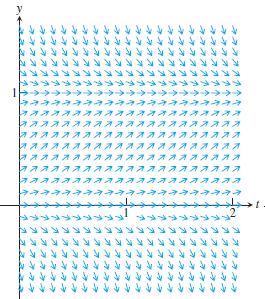
\includegraphics[width=4cm]{./Images/interpret-pvi.png}
					\caption{Representación del campo vectorial asociado a la ecuación logística $y'(t) = c y(t) (1 - y(t))$.} 
			\end{figure}
		\end{columns}			
	\end{frame}
}
		
{
	% Set the headline 
	\setbeamertemplate{headline}{
		\begin{beamercolorbox}[sep=10pt]{title} 
			\usebeamerfont{frametitle}{\color{ChetwodeBlue}Motivación: Método de Euler}
		\end{beamercolorbox}
	}
		
	\begin{frame}
			\begin{tcolorbox}[colback=ChetwodeBlue!10,colframe=ChetwodeBlue!60]
				\begin{equation}
					\begin{cases}
					w_0=y_0 \\
					h_{i} = t_{i+1} - t_i \\
					w_{i+1} = w_i + h_{i} f(t_i,w_i)
					\end{cases}
				\end{equation}
				\centering
				\fontsize{10}{8}\selectfont	
				\textbf{Método de Euler}
				\fontsize{9}{8}\selectfont								
				\begin{itemize}
					\item Mejores resultados para puntos equidistantes.
					\item Es estable, consistente y convergente.
					\item El error global de aproximación es $O(h)$.
					\item Puede parecer válido en cualquier aplicación.
				\end{itemize}
			\end{tcolorbox}	
	\end{frame}
}

{
	% Set the headline 
	\setbeamertemplate{headline}{
		\begin{beamercolorbox}[sep=10pt]{title} 
			\usebeamerfont{frametitle}{\color{ChetwodeBlue}Motivación: Ejemplo}
		\end{beamercolorbox}
	}
	
	\begin{frame}
		Considérese el siguiente problema de valores iniciales:
		
		\begin{equation*}
			\begin{cases}
			y'(t) = -4 t^3 y^2 \\
			y(-10) = 1/10001 \\
			t \in [-10,0] \\
			\end{cases}
		\end{equation*}
		
		\begin{itemize}
			\item La solución exacta es $y(t)= \frac{1}{1+t^4}$.
			\item Queremos calcular la aproximación de y en 0 con $y(0)=1$.
			\item Se va a aproximar hasta llegar a los 10000 puntos.
		\end{itemize}				
	\end{frame}
}

{
	% Set the headline 
	\setbeamertemplate{headline}{
		\begin{beamercolorbox}[sep=10pt]{title} 
			\usebeamerfont{frametitle}{\color{ChetwodeBlue}Motivación: Ejemplo}
		\end{beamercolorbox}
	}
	
	\begin{frame}
				\begin{table}[H]
					\centering
					\begin{tabular}{|| c | c | c ||}
						\hline
						\hline $N$ &  $h$ & $w_n$ \\
						\hline 100 & 0.1 & 0.00390138 \\
						\hline 1000 & 0.01 & 0.03085162 \\
						\hline 5000 & 0.002 & 0.13282140 \\
						\hline 7500 & 0.0013 & 0.18614311 \\
						\hline 10000 & 0.001 & 0.23325153 \\		
						\hline
						\hline	
					\end{tabular}
					\caption{Ejemplo de un mal comportamiento del método de Euler.}
					\label{table:euler}
				\end{table}
	\end{frame}
}


{
	% Set the headline 
	\setbeamertemplate{headline}{
		\begin{beamercolorbox}[sep=10pt]{title} 
			\usebeamerfont{frametitle}{\color{ChetwodeBlue}Motivación: Ejemplo}
		\end{beamercolorbox}
	}
	
	\begin{frame}
		\begin{figure}[H]
			\centering
			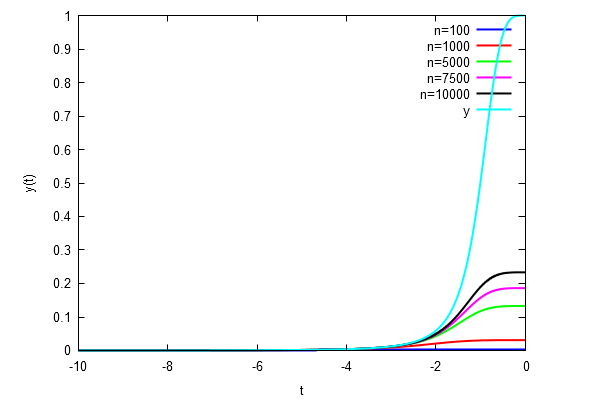
\includegraphics[width=0.7\textwidth]{./Images/eulermaxima.png}
			\label{fig:euler}
			\caption{Aproximaciones obtenidas con diferentes valores de $n$.}
		\end{figure}
	\end{frame}
}